% Options for packages loaded elsewhere
\PassOptionsToPackage{unicode}{hyperref}
\PassOptionsToPackage{hyphens}{url}
\PassOptionsToPackage{dvipsnames,svgnames,x11names}{xcolor}
%
\documentclass[
  12pt,
  letterpaper,
  DIV=11,
  numbers=noendperiod]{scrartcl}

\usepackage{amsmath,amssymb}
\usepackage{iftex}
\ifPDFTeX
  \usepackage[T1]{fontenc}
  \usepackage[utf8]{inputenc}
  \usepackage{textcomp} % provide euro and other symbols
\else % if luatex or xetex
  \usepackage{unicode-math}
  \defaultfontfeatures{Scale=MatchLowercase}
  \defaultfontfeatures[\rmfamily]{Ligatures=TeX,Scale=1}
\fi
\usepackage{lmodern}
\ifPDFTeX\else  
    % xetex/luatex font selection
  \setmainfont[Scale = MatchLowercase]{Scala Pro}
  \setsansfont[]{Scala Sans Pro}
\fi
% Use upquote if available, for straight quotes in verbatim environments
\IfFileExists{upquote.sty}{\usepackage{upquote}}{}
\IfFileExists{microtype.sty}{% use microtype if available
  \usepackage[]{microtype}
  \UseMicrotypeSet[protrusion]{basicmath} % disable protrusion for tt fonts
}{}
\makeatletter
\@ifundefined{KOMAClassName}{% if non-KOMA class
  \IfFileExists{parskip.sty}{%
    \usepackage{parskip}
  }{% else
    \setlength{\parindent}{0pt}
    \setlength{\parskip}{6pt plus 2pt minus 1pt}}
}{% if KOMA class
  \KOMAoptions{parskip=half}}
\makeatother
\usepackage{xcolor}
\usepackage[top=20mm,left=25mm,heightrounded]{geometry}
\setlength{\emergencystretch}{3em} % prevent overfull lines
\setcounter{secnumdepth}{-\maxdimen} % remove section numbering
% Make \paragraph and \subparagraph free-standing
\ifx\paragraph\undefined\else
  \let\oldparagraph\paragraph
  \renewcommand{\paragraph}[1]{\oldparagraph{#1}\mbox{}}
\fi
\ifx\subparagraph\undefined\else
  \let\oldsubparagraph\subparagraph
  \renewcommand{\subparagraph}[1]{\oldsubparagraph{#1}\mbox{}}
\fi


\providecommand{\tightlist}{%
  \setlength{\itemsep}{0pt}\setlength{\parskip}{0pt}}\usepackage{longtable,booktabs,array}
\usepackage{calc} % for calculating minipage widths
% Correct order of tables after \paragraph or \subparagraph
\usepackage{etoolbox}
\makeatletter
\patchcmd\longtable{\par}{\if@noskipsec\mbox{}\fi\par}{}{}
\makeatother
% Allow footnotes in longtable head/foot
\IfFileExists{footnotehyper.sty}{\usepackage{footnotehyper}}{\usepackage{footnote}}
\makesavenoteenv{longtable}
\usepackage{graphicx}
\makeatletter
\def\maxwidth{\ifdim\Gin@nat@width>\linewidth\linewidth\else\Gin@nat@width\fi}
\def\maxheight{\ifdim\Gin@nat@height>\textheight\textheight\else\Gin@nat@height\fi}
\makeatother
% Scale images if necessary, so that they will not overflow the page
% margins by default, and it is still possible to overwrite the defaults
% using explicit options in \includegraphics[width, height, ...]{}
\setkeys{Gin}{width=\maxwidth,height=\maxheight,keepaspectratio}
% Set default figure placement to htbp
\makeatletter
\def\fps@figure{htbp}
\makeatother

\KOMAoption{captions}{tableheading}
\makeatletter
\@ifpackageloaded{caption}{}{\usepackage{caption}}
\AtBeginDocument{%
\ifdefined\contentsname
  \renewcommand*\contentsname{Table of contents}
\else
  \newcommand\contentsname{Table of contents}
\fi
\ifdefined\listfigurename
  \renewcommand*\listfigurename{List of Figures}
\else
  \newcommand\listfigurename{List of Figures}
\fi
\ifdefined\listtablename
  \renewcommand*\listtablename{List of Tables}
\else
  \newcommand\listtablename{List of Tables}
\fi
\ifdefined\figurename
  \renewcommand*\figurename{Figure}
\else
  \newcommand\figurename{Figure}
\fi
\ifdefined\tablename
  \renewcommand*\tablename{Table}
\else
  \newcommand\tablename{Table}
\fi
}
\@ifpackageloaded{float}{}{\usepackage{float}}
\floatstyle{ruled}
\@ifundefined{c@chapter}{\newfloat{codelisting}{h}{lop}}{\newfloat{codelisting}{h}{lop}[chapter]}
\floatname{codelisting}{Listing}
\newcommand*\listoflistings{\listof{codelisting}{List of Listings}}
\makeatother
\makeatletter
\makeatother
\makeatletter
\@ifpackageloaded{caption}{}{\usepackage{caption}}
\@ifpackageloaded{subcaption}{}{\usepackage{subcaption}}
\makeatother
\ifLuaTeX
  \usepackage{selnolig}  % disable illegal ligatures
\fi
\IfFileExists{bookmark.sty}{\usepackage{bookmark}}{\usepackage{hyperref}}
\IfFileExists{xurl.sty}{\usepackage{xurl}}{} % add URL line breaks if available
\urlstyle{same} % disable monospaced font for URLs
\hypersetup{
  pdftitle={Exam Prep},
  pdfauthor={Phil 444},
  colorlinks=true,
  linkcolor={black},
  filecolor={Maroon},
  citecolor={Blue},
  urlcolor={Blue},
  pdfcreator={LaTeX via pandoc}}

\title{Exam Prep}
\author{Phil 444}
\date{2024-04-19}

\begin{document}
\maketitle

\begin{itemize}
\tightlist
\item
  The actual exam will be 6 questions taken from the questions below.
\item
  The numbers in the numerical questions will be changed, but the
  wording won't be.
\item
  For any question asking for a verbal answer (e.g., explain this
  notion, or this constraint), you should answer in about \textbf{250}
  words. These are \emph{short answer} questions, not essays, and the
  aim is to either (a) simply describe a concept or idea, or (b) present
  one reason for or against some notion. Don't try to write a five
  paragraph essay for each one!
\end{itemize}

\subsection*{Questions}\label{questions}
\addcontentsline{toc}{subsection}{Questions}

\begin{enumerate}
\def\labelenumi{\arabic{enumi}.}
\tightlist
\item
  Briefly describe the difference between what Lackey calls
  ``inflationary'' and ``deflationary'' accounts of group belief, and
  give an example of each.
\end{enumerate}

Deflationary accounts say that group beliefs are just a function of what
individuals in the group believe. E.g., the group believes p just in
case a majority of the members believe it.

Inflationary accounts say that other things than the beliefs of the
group can matter to belief. E.g., the group believes p just in case
someone in the group has evidence e, and everyone in the group thinks e
is excellent evidence for p.

\begin{enumerate}
\def\labelenumi{\arabic{enumi}.}
\setcounter{enumi}{1}
\tightlist
\item
  Explain the Conditionalisation constraint in Russell, Hawthorne and
  Buchak's paper \emph{Groupthink}.
\end{enumerate}

The constraint says that the following two operations should have the
same result.

\begin{enumerate}
\def\labelenumi{\Alph{enumi}.}
\tightlist
\item
  Combine two opinions into a group opinion, then update on some
  evidence.
\item
  Have each member of the group update on that evidence, then combine
  the two updated individual opinions into an updated group opinion.
\end{enumerate}

\begin{enumerate}
\def\labelenumi{\arabic{enumi}.}
\setcounter{enumi}{2}
\tightlist
\item
  In a local election, with 100 voters, the voters have the following
  preferences. 45 people rank the candidates ADBC (i.e., A first, D
  second, B third, C fourth); 25 rank them BCDA; 20 rank them DABC; 10
  rank them CDBA. Who would win if the voters vote sincerely, and the
  city uses first-past-the-post voting? Who would win if the voters vote
  sincerely, and the city uses ranked choice (i.e., alternate vote)
  voting? Very briefly (in a couple of sentences), which verdict do you
  think better reflects the will of the voters?
\end{enumerate}

In first-past-the-post, A gets 45, B gets 25, D gets 20, and C gets 10,
so A wins because 45 is largest.

In ranked choice, no one has a majority (i.e., 51 votes), so we
eliminate the person with the fewest votes. That's C, and all 10 of
their voters had D as second preference, so those 10 votes get added to
D. Now it's A on 45, B on 25, and D on 30 (the 20 original, and 10 new).
Still no one has a majority, so B gets eliminated. Each vote for B gets
moved to the remaining candidate who was most preferred, and in all 25
cases that's D. So now D has 55 votes and is the winner.

Either answer for the last question seems fine, since neither system
here is great. D does not have wide support - only 20\% of voters voted
for them, and the crucial votes to put them over the top came from
people who had them 3rd out of 4. On the other hand, a majority of the
voters have A outright last, and it is odd to have the worst possible
option for 55\% win the election.

\begin{enumerate}
\def\labelenumi{\arabic{enumi}.}
\setcounter{enumi}{3}
\tightlist
\item
  State Arrow's \textbf{Independence of Irrelevant Alternatives}
  condition.
\end{enumerate}

A social choice function takes the preferences of the voters as input,
and returns a social preference ordering as output.

IIA says that if you change the voters' preferences, but do not change
how any voter thinks about the relative position of A and B, then the
social preference ordering of A and B should not change. That is, if
originally A was ranked above B in the output, then the only way that
can change is if some voter changes their mind about the relative
ordering of A and B. It isn't enough if, for instance, some voters who
always had B above A change their mind about whether B or C is outright
best.

\begin{enumerate}
\def\labelenumi{\arabic{enumi}.}
\setcounter{enumi}{4}
\tightlist
\item
  Describe an example where Sen's Condition L (Liberalism) and Condition
  P (Pareto) conflict.
\end{enumerate}

A and B each have the following preferences about bedroom color.

\begin{itemize}
\tightlist
\item
  The best outcome is that their bedroom is pink, and the other person's
  is blue.
\item
  The second best outcome is that both bedrooms are blue.
\item
  The third best outcome is that both bedrooms are pink.
\item
  The worst outcome is that their bedroom is blue, and the other bedroom
  is pink.
\end{itemize}

Each person prefers having a pink bedroom to a blue bedroom, holding
fixed what the other person does. So if L says that people choose their
own bedroom color, that means they'll choose pink. But that means we'll
end up with the third best outcome; they would both prefer a world where
both bedrooms are blue.

\begin{enumerate}
\def\labelenumi{\arabic{enumi}.}
\setcounter{enumi}{5}
\tightlist
\item
  Consider an Axelrod-style Prisoners Dilemma tournament with just the
  following three strategies: Tit-for-Tat (i.e., C at move one, then do
  whatever the other person did last time); Grim Trigger (i.e., C until
  the other person plays D, then D forever); and a strategy that plays D
  until the other person plays D, then C forever. Each will play 100
  rounds against the other two. The payoffs each round are (as normal),
  5 points for playing D against C, 3 points for playing C against C, 1
  point for playing D against D, 0 points for playing C against D. How
  many points over the 200 games (i.e., 100 rounds against 2 opponents)
  will each of them end up with?
\end{enumerate}

Call the strategies TFT, GT, and Test.

TFT vs GT: Both get 300 points, since it's all C all the way.\\
TFT vs Test: Round 1, TFT plays C, Test plays D, so it's 0-5. Round 2,
TFT plays D, Test plays D, so it's 1-1. Round 3, TFT plays D, Test plays
C, so it's 5-0. So far the score is 6-6. After that they play C every
round, so it ends up 297-297.\\
GT vs Test: Round 1, GT plays C, Test plays D, so it's 0-5. Round 2, GT
plays D, Test plays D, so it's 1-1. After that, GT plays D, Test plays
C, so it's 0-5 for 98 more rounds. So GT gets 491 points, and Test gets
6 points.

Final scores: TFT 597, GT 791, Test 303.

\begin{enumerate}
\def\labelenumi{\arabic{enumi}.}
\setcounter{enumi}{6}
\tightlist
\item
  Describe an example of a \textbf{focal point} in Schelling's sense.
\end{enumerate}

A coordination game is a game where the highest priority of each player
is to do what the other(s) do, i.e., to coordinate. A focal point of a
game like this is a solution that jumps out at people as being one that
others will naturally latch on to. For example, if a group knew just
that we were all in Chicago, and wanted to meet up, heading to the Bean
would make sense; it's a focal point meaning that it's a solution to a
problem like this that people will naturally gravitate towards, and do
so in the (rational) belief that others will do so too.

\begin{enumerate}
\def\labelenumi{\arabic{enumi}.}
\setcounter{enumi}{7}
\tightlist
\item
  What is the difference between weak dominance and strict dominance?
  Describe an example where the two notions come apart.
\end{enumerate}

Option A strictly dominates B if it has a higher return whatever the
other player does.

Option A weakly dominates B if it never has a lower return than B, and
sometimes has a higher return.

In the game below, Up weakly, but not strongly, dominates Down.

\begin{longtable}[]{@{}ccc@{}}
\toprule\noalign{}
& Left & Right \\
\midrule\noalign{}
\endhead
\bottomrule\noalign{}
\endlastfoot
Up & 1,1 & 1,0 \\
Down & 0,0 & 1,1 \\
\end{longtable}

\begin{enumerate}
\def\labelenumi{\arabic{enumi}.}
\setcounter{enumi}{8}
\tightlist
\item
  In Table~\ref{tbl-dom}, what will be the result if both players use
  iterated deletion of strictly dominated strategies to decide what to
  do? (In each cell, Row's payouts are first, and Column's are second.)
\end{enumerate}

\begin{longtable}[]{@{}cccc@{}}
\caption{Game table for Q9}\label{tbl-dom}\tabularnewline
\toprule\noalign{}
& L & C & R \\
\midrule\noalign{}
\endfirsthead
\toprule\noalign{}
& L & C & R \\
\midrule\noalign{}
\endhead
\bottomrule\noalign{}
\endlastfoot
U & 1,1 & 2,0 & 2,2 \\
M & 0,3 & 1,5 & 4,4 \\
D & 2,4 & 3,6 & 3,0 \\
\end{longtable}

D strictly dominates U, resulting in Table~\ref{tbl-dom-r1}.

\begin{longtable}[]{@{}cccc@{}}
\caption{After deleting U}\label{tbl-dom-r1}\tabularnewline
\toprule\noalign{}
& L & C & R \\
\midrule\noalign{}
\endfirsthead
\toprule\noalign{}
& L & C & R \\
\midrule\noalign{}
\endhead
\bottomrule\noalign{}
\endlastfoot
M & 0,3 & 1,5 & 4,4 \\
D & 2,4 & 3,6 & 3,0 \\
\end{longtable}

After that, C strictly dominates L and R, resulting in
Table~\ref{tbl-dom-r2}.

\begin{longtable}[]{@{}cc@{}}
\caption{After deleting L and R}\label{tbl-dom-r2}\tabularnewline
\toprule\noalign{}
& C \\
\midrule\noalign{}
\endfirsthead
\toprule\noalign{}
& C \\
\midrule\noalign{}
\endhead
\bottomrule\noalign{}
\endlastfoot
M & 1,5 \\
D & 3,6 \\
\end{longtable}

Now D strictly dominates M.

So the result is Row plays D, Column plays C, and the result is Row gets
3, Column gets 6.

You just need to state the previous sentence, what's above is working
out which you can write out, but don't have to.

\begin{enumerate}
\def\labelenumi{\arabic{enumi}.}
\setcounter{enumi}{9}
\tightlist
\item
  In Figure~\ref{fig-back}, what will be the result if all players uses
  backward induction to solve the problem? (At each terminal node, the
  payouts are player 1's, then player 2's, then player 3's. Each player
  moves once; first player 1, then player 2, then player 3.)
\end{enumerate}

Every player will move L, and the result will be that P1 gets 3, P2 gets
1, and P3 gets 1.

For exam purposes, the sentence above is all you need to say.

For working out purposes, I've revised the diagram for this page so that
it shows (with double lines) what move each player will make at each
node where they could move.

\begin{figure}

\centering{

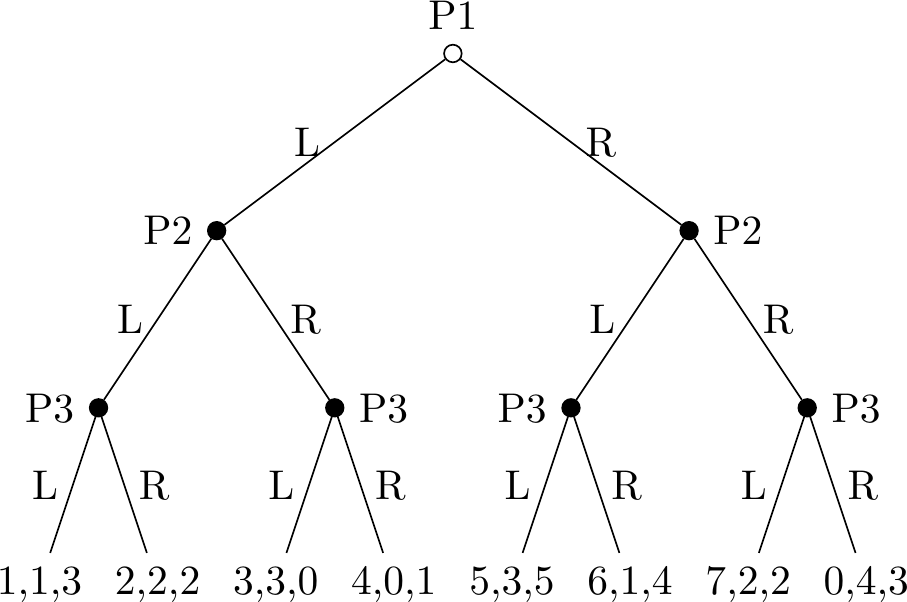
\includegraphics{sample_exam-with-notes_files/figure-pdf/fig-back-1.png}

}

\caption{\label{fig-back}Tree for Q10}

\end{figure}%

\newpage

\begin{enumerate}
\def\labelenumi{\arabic{enumi}.}
\setcounter{enumi}{10}
\tightlist
\item
  In Figure~\ref{fig-signal}, describe a separating equilbrium of the
  game.
\end{enumerate}

\begin{figure}

\centering{

\includegraphics{sample_exam-with-notes_files/figure-pdf/fig-signal-1.png}

}

\caption{\label{fig-signal}Tree for Q11}

\end{figure}%

\begin{description}
\tightlist
\item[Answer One]
Proposer plays Left if A; Right if B.

Respond plays Up if L; Down if R.
\end{description}

That's all you need to say, but to confirm it's a correct answer, ask
yourself the following four questions, all of which should get the
answer \textbf{No}.

\begin{itemize}
\tightlist
\item
  Would Proposer do better by switching if A, in this case going from
  Left if A to Right if A?
\end{itemize}

\textbf{No}. Respond plays Down if R, and if Proposer is A, plays R, and
Respond plays Down, they get 0. As it stands, if A they get 1, and 0 is
not greater than 1.

\begin{itemize}
\tightlist
\item
  Would Proposer do better by switching if B, in this case going from
  Right if B to Left if B?
\end{itemize}

\textbf{No}. Respond plays Up if Left, and if Proposer is B, plays L,
and Respond plays Up, they get 2. As it stands, if B they get 3, and 2
is not greater than 3.

\begin{itemize}
\tightlist
\item
  Would Respond do better by switching if L, in this case going from Up
  if L to Down if L?
\end{itemize}

\textbf{No}. Proposer only plays L if they are A. So the only case to
consider is the top left corner, i.e., A followed by L. In that case,
Respond gets 2 if Up, and 0 if Down, and 0 is not greater than 2.

\begin{itemize}
\tightlist
\item
  Would Respond do better by switching if R, in this case going from
  Down if R to Up if R?
\end{itemize}

\textbf{No}. Proposer only plays R if they are B. So the only case to
consider is the bottom right corner, i.e., B followed by R. In that
case, Respond gets 2 if Down, and 0 if Up, and 0 is not greater than 2.

\begin{description}
\tightlist
\item[Answer Two]
Proposer plays Right if A; Left if B.

Respond plays Up no matter what.
\end{description}

I won't go through the four questions, but you can check that the answer
is \textbf{No} in every case.

This is still a separating equilibrium, because what matters is that
\emph{Proposer} plays different things if A or if B.

\begin{enumerate}
\def\labelenumi{\arabic{enumi}.}
\setcounter{enumi}{11}
\tightlist
\item
  What is the human capital theory of the explanation of the college
  wage premium? Describe one objection to it. (You do not have to answer
  the objection.)
\end{enumerate}

According to the human capital theory of the college wage premium,
college students acquire skills by going to college, and those skills
are economically valuable. So employers pay them more because they
expect that people with these skills will provide more value (i.e.,
increase profits by a greater amount) than workers without those skills.

The slides go over three objections to this:

\begin{itemize}
\tightlist
\item
  Hard to see causal story for some kinds of degrees
\item
  Colleges don't gatekeep courses
\item
  Workers with some college background don't get a notable wage premium.
\end{itemize}



\end{document}
